%%% Druhá kapitola

\chapter{Robotický Swarm}
V češtině se také používá výraz Rojová Robotika nebo Robotický Roj, v angličtině je známý pod pojmem Swarm Robotics. Myšlenka Robotického Swarmu pochází podobně jak u Genetických Algoritmů z inspirace matkou Přírodou. Podle souhrnu \cite{swarmRobotic} popíši základní myšlenku RS.
\section{Základní vlastnosti}
Motivací pro použití RS může být chování živočichů na Zemi, když se zaměříme na skupiny živočichů jako jsou mravenci, včely, ryby a dokonce i někteří savci. Pokud bychom vložili do prostředí jednotlivce z některé ze zmíněných skupin, nebude schopen konkurovat nepřátelskému prostředí a nejspíše příliš dlouho nepřežije. Na druhou stranu, když budeme uvažovat celé společenství, tak se nám ze slabého jedince stane velmi adaptivní, odolný a rychle se vyvíjející roj. Podobnému účinku bychom se chtěli přiblížit v RS. Pro relativně jednoduchého robota, který není schopen plnit obtížný úkol, se pokusíme použít vícero robotů stejného typu, kteří společně zadaný úkol vyřeší. Navíc chceme těžit ze všech výhod hejna. \par
Jako nejčastější výhody RS oproti jednomu robotovi se nejčastěji uvádějí:
    \begin{enumerate}
        \item Paralelnost - Díky malé ceně jedince, si můžeme dovolit velkou populaci jedinců. Malou cenou jedince v ES myslíme jednoduchý robot s malou pořizovací cenou, v kontextu živočichů můžeme uvažovat množství energie, jídla pro tvorbu takového jedince. Velká populace nám umožňuje řešit vícero úkolů na ráz, také na velké ploše. Zvláště pro vyhledávací úkoly ušetříme nemalé množství času. 
        \item Škálovnatelnost - Změna velikosti populace hejna neovlivniví chování ostatních jedinců. Samozřejmě plnění úkolu bude rychlejší resp. pomalejší, ale původní hejno bude stále plnit původní úkol. Tím pádem můžeme celkem snadno upravovat velikost populace bez větší obtíží. V přírodě můžeme pozorovat, že smrt pár jednotlivých mravenců dělníků znatelně neovlivní práci celého mraveniště. Nově narození mravenci se mohou vydat do práce, zatímco zbytek mraveniště nemění činnost. 
        \item Houževnatost - Související se škálovatelností, jen v tomto případě máme na mysli necílenou změnu populace. Jak v předchozím příkladu u smrti mravenců, část robotů ES může selhat z rozličných důvodů. Zbytek hejna však bude pokračovat k cíli i když ve výsledku jim bude jeho dosáhnutí trvat o něco déle. Což se nám může vyplatit v nebezpečných prostředích. 
        \item Ekonomické výhody - Cena návrhu a konstrukce jednoduchých robotů hejna vyjde většinou levněji než jeden specializovaný robot schopný uspokojit stejné požadavky. V dnešním světě výroba ve velkém množství  vychází mnohem levněji než tvorba jednoho drahého konkrétního robota.
        \item Úspora energie - Díky menší velikosti a složitosti jednotlivých robotů vyžadují mnohem menší množství energie. Což má za důsledek, že si u nich můžeme dovolit energetickou rezervu na delší čas. Navíc když je pořizovací cena jednoho robota menší než náklady na dobití, tak díky škálovatelnosti můžeme pouze připojit nové roboty, což u drahého robota jde málokdy. 
        \item Autonomie a Decentralizace - V kontextu RS musí každý jediden hejna jednat autonomně, jedinci nejsou řízeny žádnou autoritou. Takže umí pracuje i při ztrátě komunikace. Opět se vychází z chování živých organismů. Pokud se chovají jedinci hejna dostatečně kooperativně. Tak mohou pracovat bez centrálního řízení, důsledkem toho se stává celé hejno ještě flexibilnější a odolnější, hlavně v prostředích s omezenou komunikací. Navíc hejno mnohem rychleji reaguje na změny. 
    \end{enumerate}
\par 
Mimo RS existuje i řada jiných přístupů, které se inspirovaly životem hejn v přírodě. Občas jsou zaměňovány za RS, nejčastěji se jedná o multi-agentní systémy a sensorové sítě(sensor networks). V následující tabulce jsou popsány jejich nejklíčovější vlastnosti. 
\begin{center}
    \begin{table} \resizebox{\textwidth}{!}{%
    \begin{tabular}{l l l l l @{\hspace{1.5cm}}D{.}{,}{3.2}D{.}{,}{1.2}D{.}{,}{2.3}}
            \toprule
             & Robotická hejna &  Multi-robotické systémy & Sensorové sítě & Multi-agentní systémy \\
            Velikost populace & Variabilní ve velkém rozsahu & Malá & Fixní & V malém rozsahu \\
            Řízení & decentralizované a autonomní & centralizované & centralizované & centralizované \\
            Odlišnosti & většinou homogenní & většinou heterogenní & homogenní & homogenní nebo heterogenní \\
            Flexibilita & vysoká & nízká & nízká & střední \\
            Škálovnatelnos & vysoká & nízká & střední & střední \\
            Prostředí & neznámé & známé nebo neznámé & známé & známé\\
            Pohyblivost & ano & ano & ne & vyjímečně\\
            \hline 
    \end{tabular}}
    \end{table}
    \end{center}
    Také se liší svojí aplikací Robotická hejna se nejčastěji používají v vojenských, nebezpečných úkolech a také pro řešení ekologických katastrof. Multi-robotické systémy potkáváme v transportních, skenovacích úkolech, dále pro řízení robotických fotbalových hráčů. Oproti tomu nejčetnější využití sensorových sítí zasahuje do medicínské oblasti, ochraně životního prostředí. Multi-agentní systémy zase nejvíce zasahují do řízení síťových zdrojů a distribuovaného řízení. 
\section{Použití}
Existuje několik vědeckých prací, které studují a navrhují použití RS v reálném nasazení. Některé jsem zmínil už v úvodu této práce jako například hasičům asistující roboty \cite{fireRobots}. RS se ukázala také jako dobrá aplikace u ekologický pohrom, španělští vědci testovali jejich použití při úniku ropy \cite{oilSwarm}, či hledání centra radiace \cite{radiationSwarm}. Některé neskončili u simulací a také využívali RS u fyzických robotů, u robotů na vodním povrchu \cite{aquaticRobots}. \par

\section{Řízení robotických swarmů}
Chování swarmů se řadí mezi velmi obtížné úkoly pro svět informatiky. Pro reprezentaci chování se využívá neuronových sítí, které se optimalizují pomocí nastavování vah jednotlivých perceptronů. Neboť se jedná o velký prostor vstupních informací ze sensorů a prostor pro interakci s prostředím je taktéž velmi rozsáhlý. Přímé prohledávání takto obřího prostoru nepřichází v úvahu, proto v poslední získavají na oblibě evoluční algoritmy. Mezi nejvíce používané patří Evoluční strategie, či Genetické programování \par 

\subsection{Genetické programování a stromy chování}
V práci "Evolving behaviour trees for Swarm robotics" \cite{jonesevolving} Alan F T Winfield s kolegy podporují myšlenku evoluce chování v hejnové robotice. Pro řízení navrhují vcelku zajímavé využití stromů chování(SC)(Behaviour tree), které mají uplatnění především v herním průmyslu pro chování charakterů, které nejsou ovládány hráčem. Jako optimalizační algoritmus zvolili Genetické programování. 
\par
Strom chování je strom, jehož listy intereagují s prostředím, vnitřní vrcholy spojují tyto akce dohromady a tvoří rozhodovací a závislostní pravidla. Celý strom je vyhodnocován v pravidelných intervalech, v práci se značí jako "tick". Opírají se o článek \cite{shoulson2011parameterizing},kde bylo ukázáno, že SC může plnohodnotně reprezentovat konečné automaty, dokonce i když budeme používat pravděpodobností konečné automaty. Jako jedince z hejna zvolili Kilobot, které byl představen Rubenstein \cite{Kilobots}. Kilobot se pohybuje pomocí dvou vibračních motorů, komunikují přes infračervený kanál, v prostředí se orientují pomocí foto detektoru a signalizují pomocí LED diod s barevným spektrem. Následující části zjednodušují komunikaci s efektory robota a nad nimi optimalizováno SC. 
\par
\begin{center}
    \begin{tabular}{l  l  l@{\hspace{1.5cm}}D{.}{,}{3.2}D{.}{,}{1.2}D{.}{,}{2.3}}
        \toprule
        Efektor/Sensor & Read or Write & Popis \\
        \midrule
        motor & W & vypnut, vřed, vlevo, vpravo \\
        přídavná paměť & R\&W & libovolná hodnota \\
        vysílač signálu & R\&W & vysilá při větší hodnotě než 0.5\\
        přijímač signálu & R & 1 pokud přijímá signál \\
        detektor potravy & R  & 1 pokud světelný snímač vidí potravu\\
        nosič jídla & R & 1 pokud nese jídlo \\
        hustota robotů & R & hustota Kilobotů v blízkosti \\
        $\delta hustota$ & R & změna v hustotě \\
        $\delta vzdálenost_{potrava}$ & R & změna ve vzdálenosti k potravě \\
        $\delta vzdálenost_{hnízdo}$ & R & změna ve vzdálenosti k hnízdu \\ 
        \bottomrule
    \end{tabular}
\end{center}
\par
Tyto akce pak odpovídají listům v SC, vnitřní vrcholy mohou být následujících kompoziční: \textbf{seqm}, \textbf{selm}, \textbf{probm} a tyto mohou mít 2 až 4 syny. Informace procházející mezi vrcholy mohou být následujícího druhu \textit{success}, \textit{failure},\textit{running}. Zpracovávají informace následujícím způsobem posílají tick do každého syna dokud od nějakého nepřijde hodnota \textit{failure} nebo tick proběhne na všech synech, pokud proběhne úspěšně tick u všech synů vrací \textit{success}, \textit{failure} jinak. Oproti tomu \textbf{selm} vysílá tick, dokud mu nějaký syn nevrátí hodnotu \textit{success} nebo všichni synové provedli tick, pokud se nevrátí jediná hodnota \textit{success}, tak vrací \textit{failure}, v opačném případě \textit{success}. Od obou se liší \textbf{probm}, ten s danou pravděpodobností vybere jednoho syna a vrátí jeho odpověď. Vrchol, který má alespoň jednoho syna se statusem \textbf{running} vrací stejnou hodnotu. \par
Vrcholy jen s jedním synem patří do jedné z následujících kategorií: \textbf{repeat}, \textbf{successd}, \textbf{failured}. Vrchol \textbf{repeat} vrací tick svým synům, s daným početem pokusů, dokud nedostane hodnotu \textit{success}. Následující dva vrcholy vrací konstatní odpověď na tick dle svého jména, i přesto pošlou tick svému následníkovi. \par
Poslední skupinu vrcholu tvoří tzv. akční vrcholy \textbf{ml},\textbf{mr},\textbf{mf}, což ve stejném pořádí jsou: zatoč vlevo, zatoč vpravo, jeď kupředu. Vrcholy pohybu při první ticku vrací \textit{running} při druhém \textit{success} K akčím vrcholům také patří \textbf{if}, který implementuje porovnávání synů a vrací \textit{success}, pokud porovnání platí. Poslední z akčních vrcholů je \textbf{set}, který nastavuje danou hodnotu synům. 
\par
V prostředí jsou s konstantní frekvencí prováděny tzv. update cykly. Jeden takový cyklus se skládá z: 
\par
\begin{enumerate}
    \item Spočítají se hodnoty v synech z vysílaných signálů a prostředí. 
    \item Na SC je proveden tick, což čte a zapisuje hodnoty do synů. 
    \item Pohybové motory jsou aktivovány a vysílání je upraveno, oboje dle zapsaných hodnot do synů.
\end{enumerate}
\par 
Jako zátěžový test používají obvyklý scénář, který spočívá v hledání potravy a odvážení potravy zpět do hnízda. Fitness se hodnotí podle vzdálenosti doneseného jídla, čím blíže k hnízdu tím lépe. Jako optimalizační metodu vybrali genetické programování a používají DEAP knihovnu \cite{deap}. \
Celá populace velikosti $n_{pop}$ je ohodnocena fitness, každý jedinec se hodnotí podle 10 simulací, každá simulace má jinou startovní konfiguraci. Roboti startují vždy na poli o velikosti 5x5, jejich orientace je vybírána náhodně. Běží 300 simulovaných sekund, frekvence update cyklu 8Hz pro vnímání prostředí a u ovladačů s 2Hz. Používané Genetické programování implementuje elitimus přenáš $n_{elite}$ nejlepších jedinců do další generace, zatímco zbylá část je zvolena pomocí turnajovou selekcí s velikostí $t_{size}$. A křížící(rekombinační) operátor, který kříží části stromů, je aplikován s pravděpodobností $p_{xover}$ na všechny páry vybrané turnajovou selekcí. Na vzniklé páry se aplikují 3 mutační operátory. \par
\begin{enumerate}
    \item S pravděpodobností $p_{mutu}$ je náhodný vrchol stromu vyměněn za nový náhodně vytvořený 
    \item S pravděpodobností $p_{muts}$ je náhodná větev stromu aje  vyměnena za náhodně zvolený terminál(vyskytující se na této větvi)
    \item S pravděpodobností $p_{mutn}$ je náhodný vrchol vyměnen za nový, ale se stejným počtem argumentů
    \item S pravděpodobností $p_{mute}$ je náhodná konstanta vyměněna za jinou náhodnou hodnotu
\end{enumerate}
Krom simulace 25 nezávislých běhů evoluce. Také byly otestovány algoritmy na reálných strojích, vytrénované chování bylo otestováno 20 běhy s rozdílnou startovací pozicí a ohodnoceni stejnou fitness. 
\par 

\begin{center}
    \begin{tabular}{l  l  l@{\hspace{1.5cm}}D{.}{,}{3.2}D{.}{,}{1.2}D{.}{,}{2.3}}
        \toprule
        \textbf{Konkrétní nastavení parametrů} \\
        \hline
        Parametr & Hodnota & Popis\\
        \midrule
        $n_{gen}$ & 200 & Generace\\
        $t_{test}$ & 300 & Délka testu ve vteřinách \\
        $n_{pop}$ & 25 & Velikost populace \\
        $n_{elite}$ & 3 & Velikost Elity \\
        $p_{xover}$ & 0.8 & Pravděpodobnost křížení \\
        $p_{mutu}$ & 0.05 & Pravděpodobnost výměny podstromu \\
        $p_{muts}$ & 0.1 & Pravděpodobnost scvrknutí podstromu \\
        $p_{mutn}$ & 0.5 & Pravděpodobnost výměny vrholu \\
        $p_{mute}$ & 0.5 & Pravděpodobnost výměny konstanty \\
        \bottomrule
    \end{tabular}
\end{center}
\par
Výsledky simulace byly více než uspojivé maximální fitness, v simulační části si hejno vedlo o trochu lépe 0.075 z maximální hodnoty 0.12(minimum 0) a co se týče reálného nasazení vygenerovaného chování 0.058. Což opravdu není velký rozdíl, když přihlédneme k tomu, že evoluce probíhala čístě na simulační rovině. Následující graf zachycuje výslednou fitness. 
\par
\begin{center}
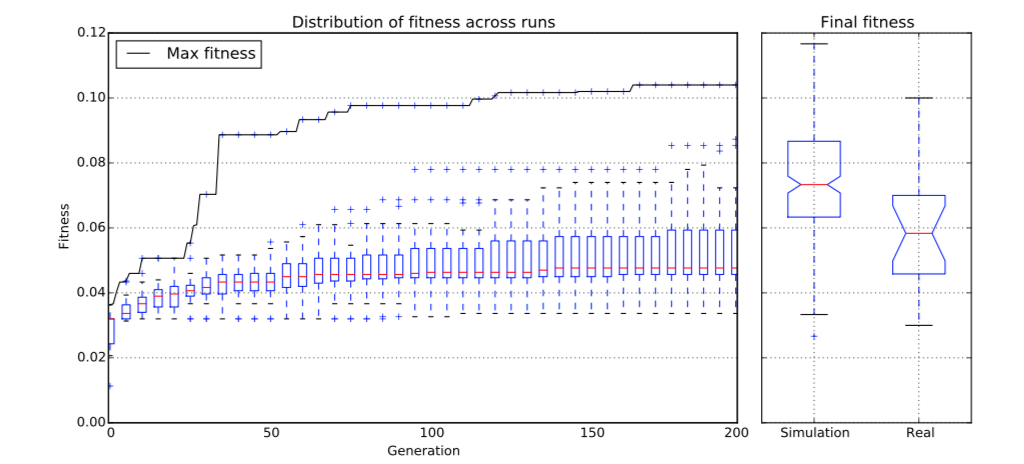
\includegraphics[scale=0.8  ]{../img/kilobotsGraph.png}
\end{center}

\subsection{Genetické algoritmy a neuronová síť}
Cagri a Yalcin používají ve své práci \citep{yalcin2008evolving} práci neuronových sítí místo SC a pro nastavení vah Getického algoritmu. Shodují se s Winfieldem a jeho kolegy, že evoluce chování robotického hejna přináší zajímavých strategií, která mohou být mnohem komplexnější než explicitně vytvořené chování. Také však popisují obtížnosti použití Evoluce, zvláště volbu Evolučního algoritmu a efektivnost celého výpočtu. 
\par
Využívají již existujícího simulátoru Cobot2D, pro všechny experimenty bylo použita mapa bez překážek velikosti 400x400. Roboti se pohybují pomocí dvou-kolečkových motorů, orientují se 4 infračervenými sensory a 4 zvukovo-směrovými sensoru, v jejich středu je umístěn všesměrový zvukový vysílač. Vysílače mají pevný rozsah kruhu vysílání a dynamickou sílu. Zvukové sensory se rozhodují pouze podle signálů, jejichž vysílače spadají do $90^\circ$ výseče od sensoru a také jejich vzdálenost musí být menší než daná konstanta. Síla signálu se zmenšuje směrem od vysílače a sensory vrací součet sil signálů. Infračervené sensory úsečku dané velikosti a orientace vzhledem k robotovi, a vrací vzdálenost k nejbližšímu průsečíku. Aby se simulace přiblížila, co nejvíce reálnému nasazení, tak jsou generovány náhodné šumy pro každou interakci s prostředím. Pro ovládání robota byla navržena neuronová síť, která má 8 vstupů(4 pro infra-sensory a 4 pro zvukové) a 3 výstupy a není zde žádná skrytá vrstva. Nákres robota a jeho ovládací neuronové sítě, můžete vidět na obrázku. \par
\begin{center} 
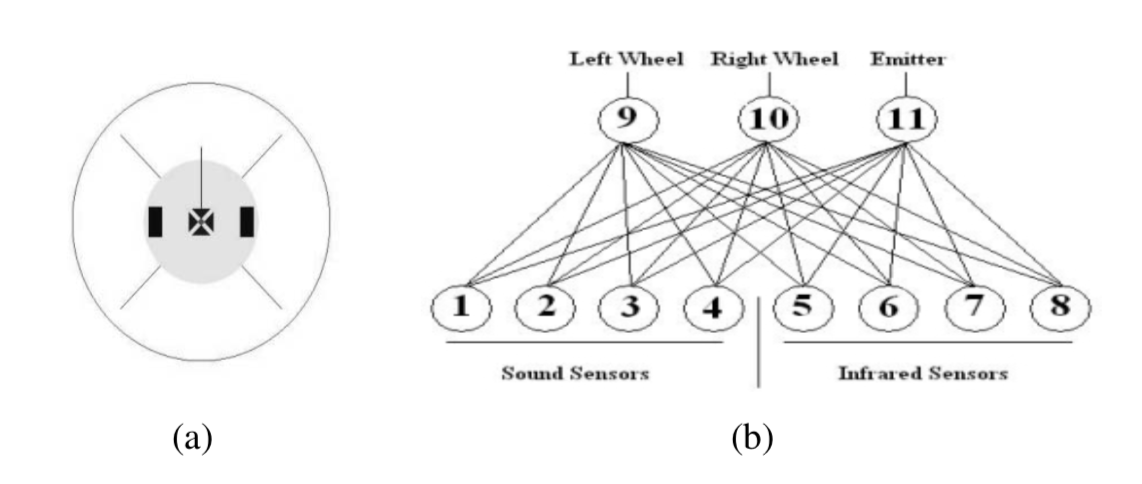
\includegraphics[scale=0.5]{../img/Cobot.png}
\end{center}
\par
Genetický algoritmus, jak jej nazývají, má následující podobu.\par 
\ \newline
\textbf{Genetický algoritmus}:
\begin{enumerate}
    \item inicializuj populace P 100 jedinců a každý jedinec reprezentován váhovým vektorem
    \item nastav všem váhovým vektorům z populace náhodné floating point hodnoty v intervalu $\in (-1,1)$ 
    \item $G_{current}$ nastav na 0(,id generace)
    \item dokud $G_{current} < 100$ prováděj \begin{enumerate}
        \item Pro každý vektor $w \in P$ \begin{enumerate}
            \item vytvoř 5 simulací prostředí s 10 roboty a orientovanými náhodně
            \item přiřad každému roboty jako ovladač neuronovou síť s váhami w
            \item spust simulaci pro 5000 kroků v každé imulci
            \item každé simulaci spočítej fitness pro skupinku robotů
            \item průměr z vypočítaných fitness z předchozího kroku přiřaď jako fitness vektoru w
        \end{enumerate} 
    \item setřiď vektory podle jejich fitness 
    \item nejlepších 20 zvol jako elitu $P_{e}$
    \item zvol náhodně 80 vektorů $P_c$ a aplikuj na ně křížení(prohazuje 1/3 vektoru a shodné páry)
    \item náhodně 40 vektorů z $P_c$ a aplikuj mutační operátor(přičtení náhodného čásla z $(-1,1)$)
    \item jako P zvol $P_c \cup P_e$
    \item $G_{current} += 1$
    \end{enumerate} 
    \item Vrať jedince, který má z P největší fitness    
\end{enumerate} 
\par 
\textbf{Fitness Funkce}: První použitá $fitness_1$ z tohoto experimentu, obrácená hodnota průměrné vzdálenosti do středu robotické skupiny. 
\par
\begin{center}
\textbf{$fitness_1 = \frac{1}{\frac{1}{n\sum\limits_{r=1}^{n} d{rc}}} $}
\end{center}
\par 
Kde $n$ je počet robotů v robotické skupině, $r$ je robotův index, $d_{rc}$ je euklidovská vzdálenost mezi $r$ středem robotické skupiny $c$. 
\par
Druhá $fitness_2$ používá metodu "inverse of hierarchical social entropy" Balche \citep{balch2000hierarchic}. Tato metoda počítá kompaktnost skupiny, tím že hledá každý možnou skupinku(cluster) pomocí změn maximální vzdálenosti $h$ mezi jedinci ze stejného clusteru. Přidávají ještě rozšíření od "Shannon's information entropy", jenž používá pevné $h$. Toto rozšíření je definováno: 
\par 
\begin{center}
\textbf{$H(h)=-\sum\limits_{k=1}^{M} p_k log_2(p_k)$}
\end{center}
\par 
H se nazývá entropie, $p_k$ je proporce jedince z clusteru $k$, $M$ je počet clusterů pro dané $h$. Konečně celý předpis daný Balchem vypadá následovně: 
\par
\begin{center}
\textbf{$fitness_2 = \frac{1}{\int_{0}^{\infty}H(h)dh}$}
\end{center}
\par 
Ve výsledku se ukázalo použití neuronových sítí a genetického algoritmu jako vhodného prostředku pro učení robotického hejna. Neboť se vygenerované chování se obstojně shlukují do úzkých skupin. Definují další tzv. cost funkci pro měření úspěchu nalezených chování, aby mohli porovnávat funkce fitness. A $fitness_2$ se ukazuje jako účinější. 
%% https://link.springer.com/article/10.1007/s11721-012-0075-2 \par

